\section{Problems}
\subsection{Sweat is entering the Housing}
The first watch broke down after nearly 1 year. After opening the Housing the Problem was very obvious. Sweat was entering the Housing and corroded the PCB and the mounted parts.
\begin{center}
  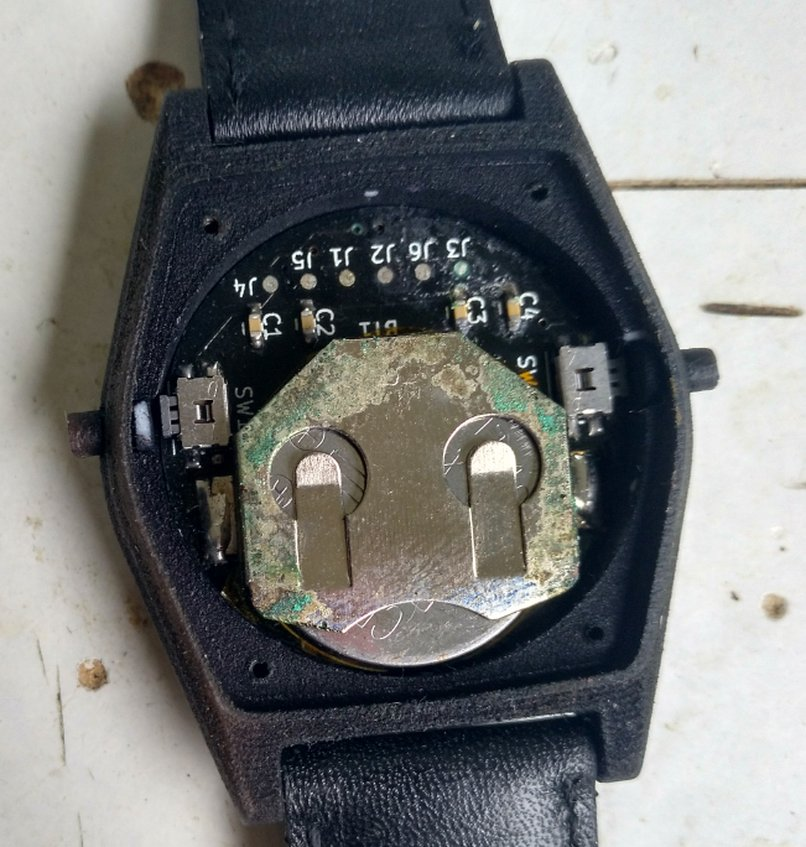
\includegraphics[width=0.5\textwidth]{../Pictures/ProbCorr1.jpg}
\end{center}
\subsubsection{Cleaning the PCB and adding something to absorb the moisture}
As a solution i tried to clean the PCB with Isopropanol and glued some rice to the PCB to absorb the moisture, that helped only for about a week and the Watch stopped working again. So that is not the best solution, but is is an extraordinary try ;-)
\begin{center}
  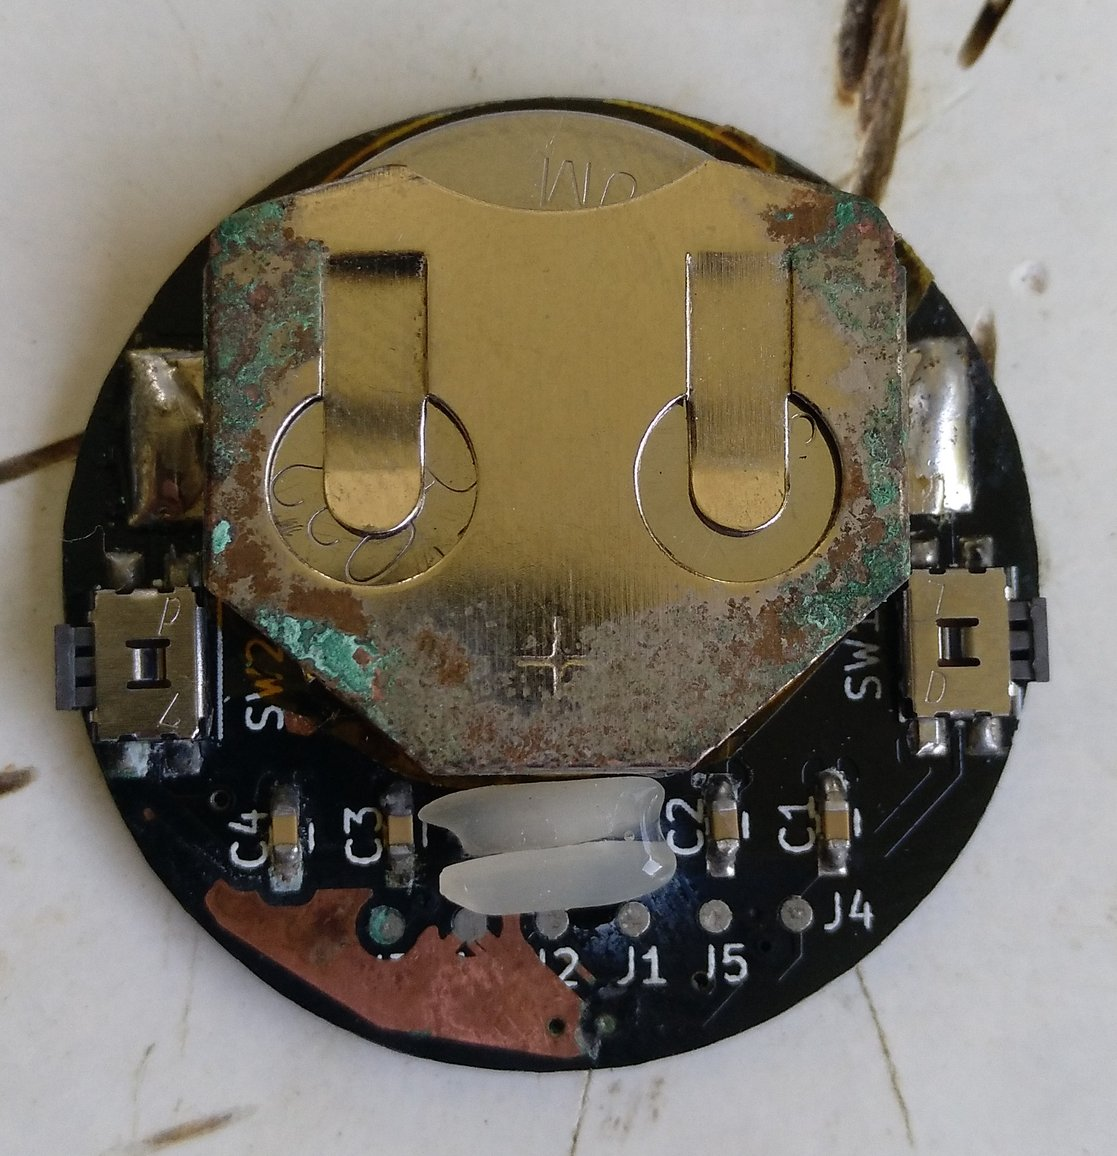
\includegraphics[width=0.5\textwidth]{../Pictures/ProbCorrSol1.jpg}
\end{center}
\subsubsection{adding isolation Tape between the lid and the housing}
The second solution was to add Tape, which is originally designed to be used to seal threads, between the housing and the lid.\
That worked out a little bit better, but the Watch also stopped working after a few weeks. 
\subsubsection*{Analyzing the Watch again}
After analyzing it again the PCB seemd to be ok. The PCB was only a little damaged from the first sweat attack.
The Problem was that the time stopped to run, but another point was that the LEDs wont go off anymore. 
But it was possible to set the time. 
So the conclusion is that the clock which is run by the crystal stopped running.
\subsubsection{Adding clear Nailpolish to guard the Crystal}
The next attempted solution was to add clear Nailpolish to the PCB, so the crystal is completely covered. This is an attempt to stop moisture from crawling below the crystal and stopping the clock.